\documentclass[12pt,journal,comsoc, letterpaper, twocolumn]{IEEEtran}
\usepackage{graphicx}
\usepackage[utf8]{inputenc}




\ifCLASSINFOpdf
 
\else
 
\fi



\begin{document}


\title{Low Power Routing Protocol For Wireless SN \newline  {\normalsize Systemic Review}} 
 
 \author{\textit{{\small Muhammad Ali }}       
 
  \textit{{\small }}        
\
\thanks{}
\thanks{}
\thanks{}}
\maketitle


\begin{abstract}
and present delays while trusting that the following bounce will wake up. In this paper,  we present ORW, a reasonable artful steering plan for remote sensor systems. In a duty-cycle setting, packets are routed to set of potential collectors, packets sent by the neighbor that awakens the first node effectively get the packets. This decreases delay and vitality utilization by using all neighbors as potential forwarders. Besides, this builds strength to remote interface elements by misusing spatial assorted variety. Our outcomes demonstrate that ORW diminishes radio obligation cycles by and 



\end{abstract}


\begin{IEEEkeywords}
RPL Upward Routing, Downward Routing (DR), IOT, LLN
\end{IEEEkeywords}










\section{Introduction}


and present delays while trusting that the following bounce will wake up. In this paper,  we present ORW, a reasonable artful steering plan for remote sensor systems. In a duty-cycle setting, packets are routed to set of potential collectors, packets sent by the neighbor that awakens the first node effectively get the packets. This decreases delay and vitality utilization by using all neighbors as potential forwarders. Besides, this builds strength to remote interface elements by misusing spatial assorted variety. Our outcomes demonstrate that ORW diminishes radio obligation cycles by and 

 





\section{LITERATURE REVIEW}





\section{METHODS}



 


 \textbf{ Inclusion criteria excluded}
 \newline


\begin{itemize}  
\item RPL Downward routing
\item	Short intro of RPL 
\item	Studies on priors Testbed of RPL Upward and downward Routing
\item	RPL Mobility 
\item Challenges in RPL 
\item	Support for RPL DR (improvement, but why)
\item	low power Lossy network (LLN)
\item	Rpl downward routing problem due to upward routing 
\newline


\end{itemize} 






\begin{figure*}
\begin{center}
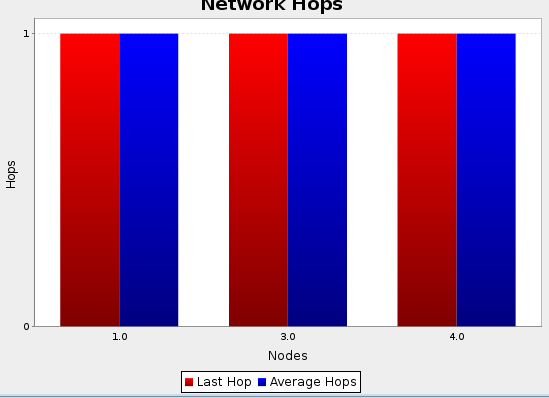
\includegraphics[width=0.7\textwidth=0.5]{RPL1}

Graph 1 Shows the Network Hops: last hops and Received hops. in this graph Red color show the last hop and the blue color shows the received hops. 

\end{center}
\end{figure*}
 





\section{RESULTS}


 


\subsubsection{RPL DR need solution}	

Even though RPL centers essentially around upward traffic conveyance, numerous basic sensor checking applications, for example, Advanced metering infrastructure, requires meters to be 'arranged' or impelled the descending way. Additionally, the utilization of TCP, as well as the application layer, ACKs, will order bi-directional availability [2]



\section{Conclusion}

I found 20 articles from 2016 to 2020 from which 5 articles are included in our paper, even though the 




















\ifCLASSOPTIONcaptionsoff
  \newpage
\fi



\begin{thebibliography}{1} 

\bibitem{IEEEhowto:kopka}
Zhong, Xiaoyang, and Yao Liang. "Scalable Downward Routing for Wireless Sensor Networks Actuation." IEEE Sensors Journal 19.20 (2019): 9552-9560


\bibitem{IEEEhowto:kopka}
Min, Soon-Woong, Sang-Hwa Chung, and Yu-Vin Ha. "An Improved Mobility Support Mechanism for Downward Traffic in RPL." 2018 Tenth International Conference on Ubiquitous and Future Networks (ICUFN). IEEE, 2018.














\end{thebibliography}










\end{document}


